% Orthogonal projection, drawn exactly: the plane z = 0 stands for the span of the ten parameter
% directions (drawn as two), F is the learned correction, its orthogonal projection onto the plane
% is the part a parameter change could also produce (removed), F minus that projection is kept.
% Oblique projection of 3D coordinates; the right angle is a true 3D right angle.
\documentclass[border=8pt]{standalone}
% Shared preamble of the TikZ slide figures. Role colours match style.py.
\usepackage[T1]{fontenc}
\usepackage[scaled]{helvet}
\renewcommand\familydefault{\sfdefault}
\usepackage{amsmath}
\usepackage{tikz}
\usetikzlibrary{arrows.meta,calc,decorations.pathmorphing,positioning}
\definecolor{cbase}{HTML}{D55E00}   % physics model
\definecolor{caug}{HTML}{0072B2}    % augmented model, no projection
\definecolor{cproj}{HTML}{009E73}   % augmented model with projection
\definecolor{cink}{HTML}{222222}
\definecolor{cmuted}{HTML}{6B6B6B}

\begin{document}
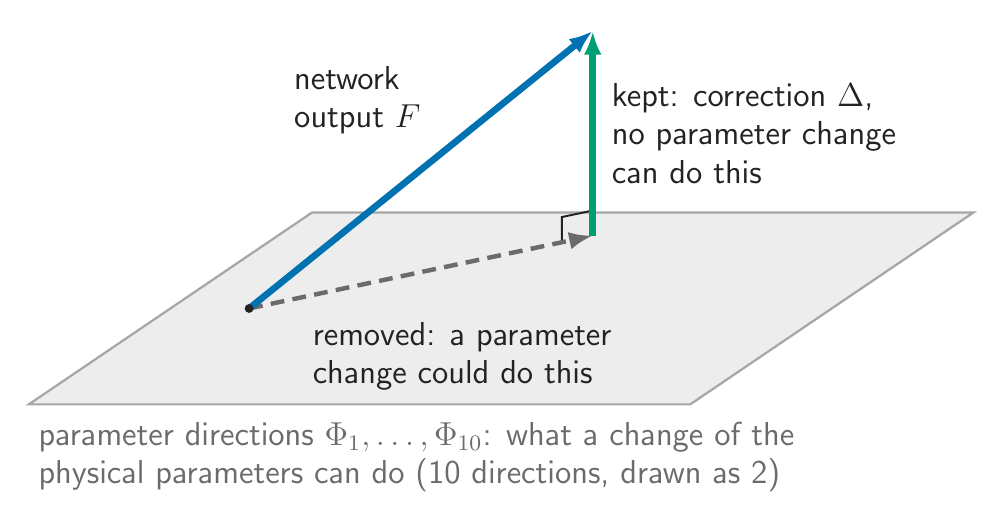
\begin{tikzpicture}[
    x={(1cm,0cm)}, y={(0.62cm,0.42cm)}, z={(0cm,1cm)},
    >={Latex[length=3mm]},
    lbl/.style={font=\large, text=cink, align=left},
  ]
  \coordinate (O) at (0.6, 0.5, 0);
  \coordinate (F) at ($(O)+(3.0, 2.2, 2.6)$);
  \coordinate (Pf) at ($(O)+(3.0, 2.2, 0)$);
  % the plane
  \filldraw[fill=cmuted!12, draw=cmuted!60, line width=0.8pt]
    (-0.4,-2.4,0) -- (8.0,-2.4,0) -- (8.0,3.4,0) -- (-0.4,3.4,0) -- cycle;
  \node[font=\large, text=cmuted, align=left, anchor=north west]
    at ($(-0.4,-2.4,0)+(0cm,-0.1cm)$)
    {parameter directions $\Phi_1,\dots,\Phi_{10}$: what a change of the\\physical parameters can do (10 directions, drawn as 2)};
  % right-angle marker at the foot of the perpendicular
  \coordinate (A) at ($(Pf)!0.09!(O)$);
  \draw[cink, line width=0.7pt] (A) -- ($(A)+(0,0,0.32)$) -- ($(Pf)+(0,0,0.32)$);
  % removed: in-plane part
  \draw[->, line width=1.6pt, draw=cmuted, dash pattern=on 5pt off 3pt] (O) -- (Pf);
  % kept: perpendicular part
  \draw[->, line width=2.4pt, draw=cproj] (Pf) -- (F);
  % the learned correction
  \draw[->, line width=2.4pt, draw=caug] (O) -- (F);
  \fill[cink] (O) circle (1.6pt);

  \node[lbl, anchor=south east] at ($(O)!0.55!(F)+(-0.1,0,0.15)$) {network\\output $F$};
  \node[lbl, anchor=west] at ($(Pf)!0.5!(F)+(0.12,0,0)$)
    {kept: correction $\Delta$,\\no parameter change\\can do this};
  \node[lbl, anchor=north] at ($(O)!0.62!(Pf)+(0cm,-0.62cm)$)
    {removed: a parameter\\change could do this};
\end{tikzpicture}
\end{document}
